\frame[plain]{\titlepage}
% \frame{\frametitle{Outline}\tableofcontents}

\section{Introduction}

\begin{frame}
    \frametitle{Introduction}
    
    In the presentation, I would first introduce Monte Carlo Integration, which requires enormous random sample. Then we introduce common ways of sampling from a given distribution, including Transformation method, Accept-rejection method, and Markov Chain Monte Carlo Algorithm. In each method I would show code implementation, analyse the pros and cons, and a brief proof.
    
\end{frame}
\section{Monte Carlo Integration}
\begin{frame}
    \frametitle{MC Integration}
    Suppose we want to evaluate an integral
    \begin{align*}
    \int_D \phi(x) d x
    \end{align*}
    for which there is no closed analytic solution. If the integrand has the form
    \begin{align*}
    \phi(x)=\tilde{\phi}(x) f(x)
    \end{align*}
    for some density function \(f\), then the integral has the form:
    \begin{align*}
    \int_D \phi(x) d x=\int_D \tilde{\phi}(x) f(x) d x=E[\tilde{\phi}(X)]
    \end{align*}
    where \(\mathrm{X}\) is an RV with \(\mathrm{PDF} f\). 

    

\end{frame}
\begin{frame}
    % \frametitle{<title>}
    \frametitle{MC Integration}
    If we know how to simulate realisations of \(X\), say \(x^{(1)}, \ldots, x^{(n)}\), then we have an estimate
    \begin{align*}
    \int_D \phi(x) d x=E[\tilde{\phi}(X)] \approx \frac{1}{n} \sum_{i=1}^n \tilde{\phi}\left(x^{(i)}\right)=\hat{I}
    \end{align*}
    Also, the variance should be
    \begin{align*}
        \operatorname{Var}(I) &= \frac{1}{n^2} \sum_{i=1}^n \operatorname{Var}\left(\tilde{\phi}\left(x^{(i)}\right)\right) \\
        &\approx \frac{1}{n(n-1)} \sum_{i=1}^n \left(\tilde{\phi}\left(x^{(i)}\right) - \hat I\right)
    \end{align*}
    % \vspace{1em}
    So it is crucial to generate sample from a specific distribution.

    

\end{frame}
\section{Transformation method}
\subsection{Algorithm}

\begin{frame}
    \frametitle{Derivation of the Algorithm}

    The easiest distribution for computer to generate is \(\operatorname{Unif}[0,1]\). If \(X\) owns CDF \(F(\cdot)\), Then \(F(X) \sim \operatorname{Unif}[0.1]\). By \textit{inversion}, setting \(X \sim F^{-1}(U)\), which \(U \sim \operatorname{Unif}[0,1]\). Then From the uniform distribution sample we can generate sample follows \(F(\cdot)\).
    \vspace*{1em}

    Consider discrete random variable, simply left
    \[F^{-1} (u) = \min\left\{x:F(x)\geq u\right\}\]
    And the algorithm goes on as continuous situation.

\end{frame}
\subsection{Pros and Cons}
\begin{frame}
    \frametitle{Pros and Cons}
    \begin{columns}
        \column{0.5\textwidth}
        \begin{block}{Pros}
            \begin{itemize}
                \item Almost Easiest way to generate a sample
                \item ?
            \end{itemize}
        \end{block}
        
        \column{0.5\textwidth}
        \begin{block}{Cons}
            \begin{itemize}
                \item The CDF is not invertible,i.e. PDF \(f(\cdot) = 0\) somewhere.
            \end{itemize}
        \end{block}

        
    \end{columns}
    
\end{frame}
\section{Accept-Reject method}
\subsection{Algorithm}

\begin{frame}
    \frametitle{Intuition}

    % require graph
    \begin{figure}
        \begin{center}
            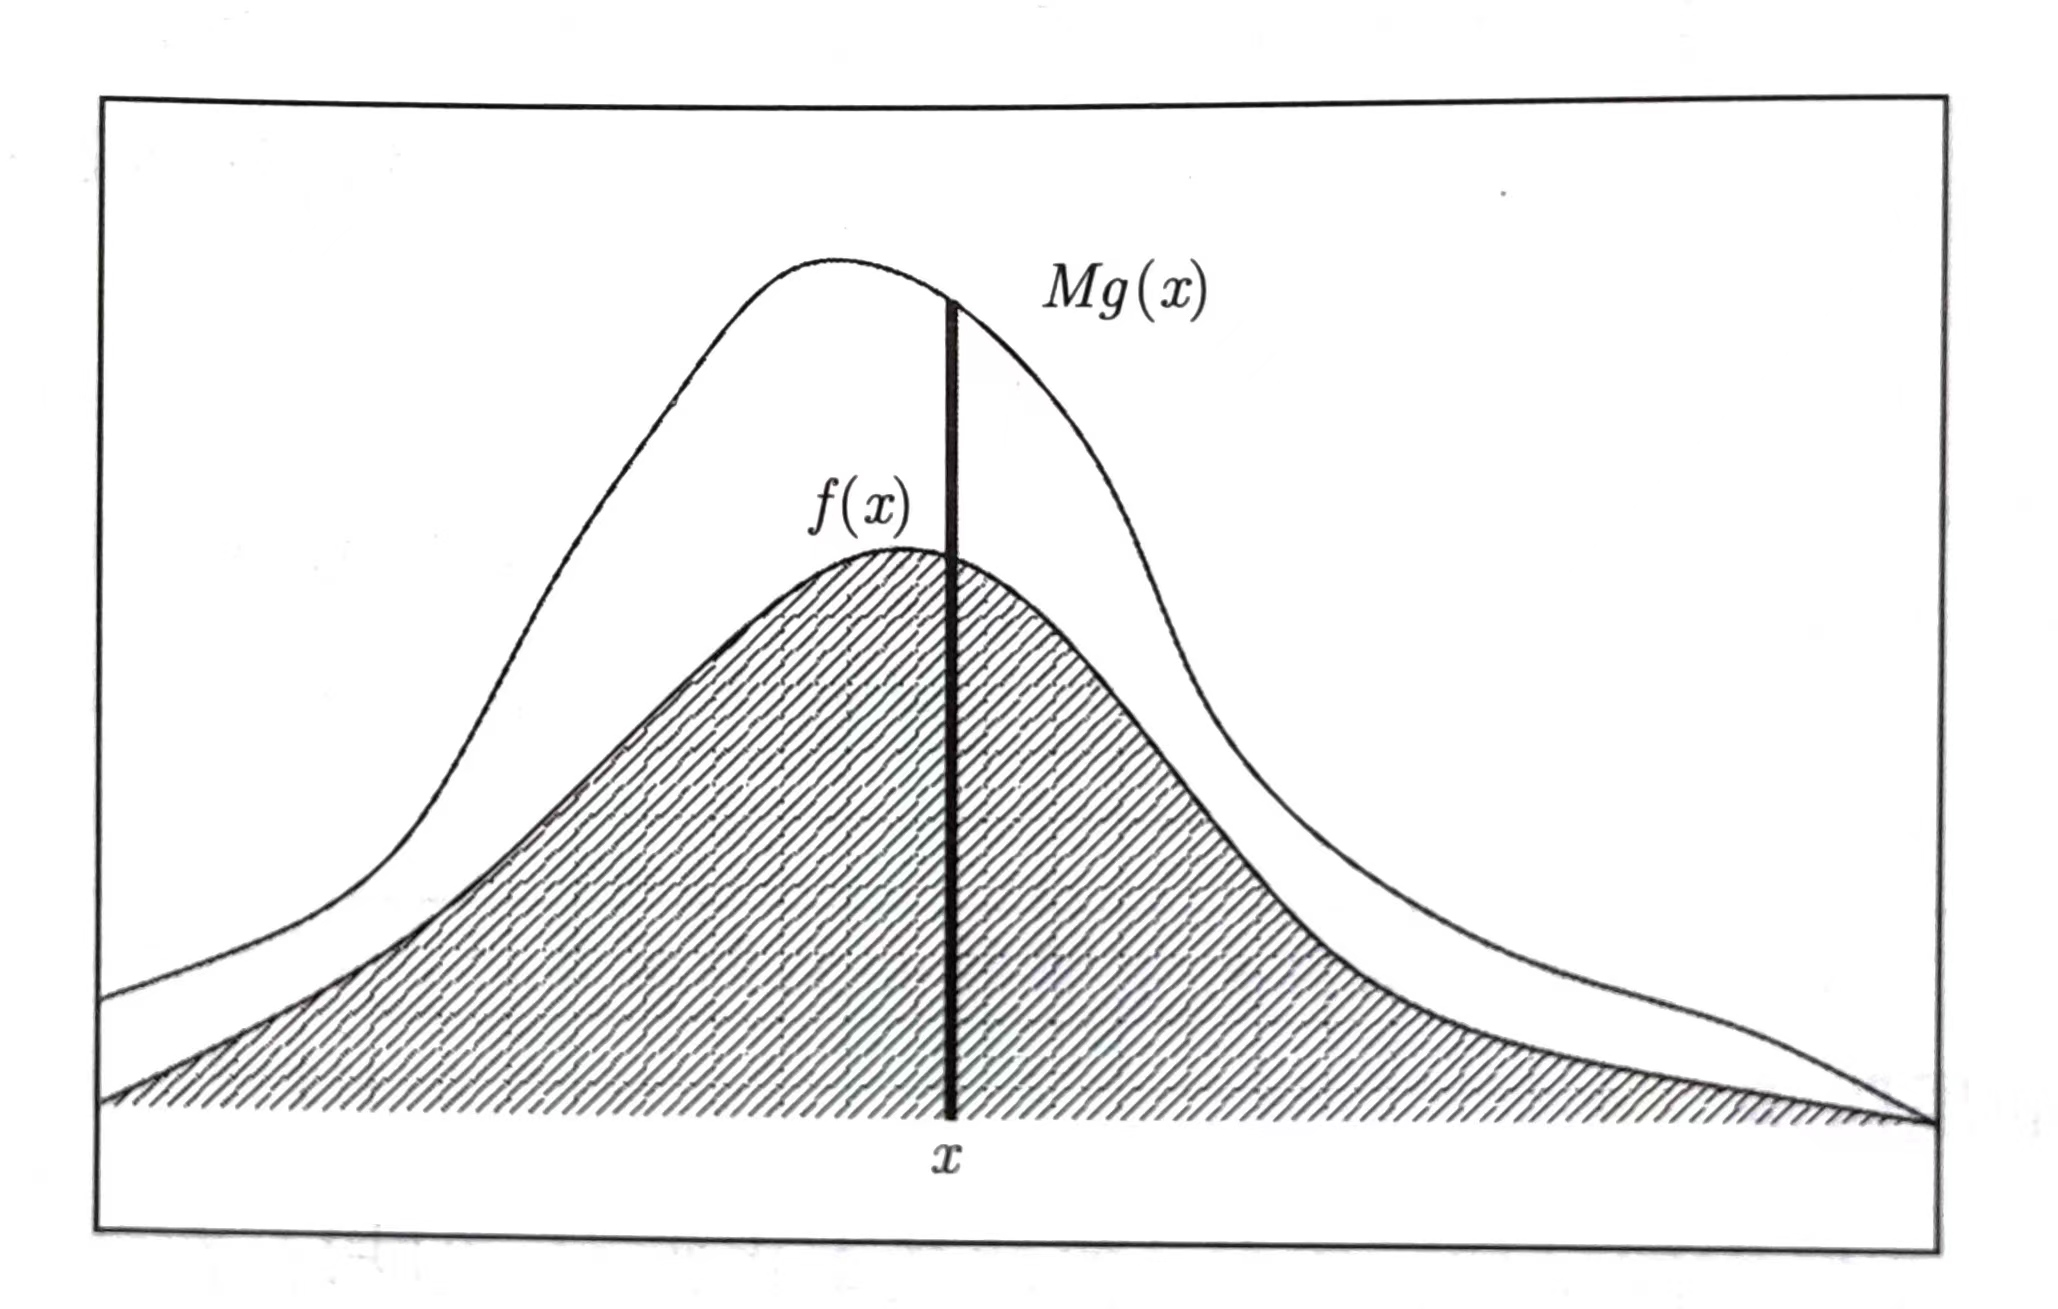
\includegraphics[width = .58\linewidth]{image1.png}
        \end{center}
    \end{figure}

    \begin{itemize}
        \item \(f(x)\): object function
        \item \(g(x)\): proposal function
        \item \(M\): auxiliary constant
        \item Make sure that \(Mg(x)\geq f(x)\) for all \(x \in \Omega\)
    \end{itemize}

\end{frame}

% \begin{frame}{Algorithm}<presentation:0>
%     \scriptsize
%     \begin{algorithm}[H]
%         \KwData{this text}
%         \KwResult{how to write algorithm with \LaTeX2e }
%         initialization\;
%         \While{not at end of this document}{
%             read current\;
%             \eIf{understand}{
%             go to next section\;
%             current section becomes this one\;
%             }{
%             go back to the beginning of current section\;
%             }
%         }
%         \caption{How to write algorithms
%         (copied from \href{https://en.wikibooks.org/wiki/LaTeX/Algorithms}{here})}
%         \end{algorithm}
% \end{frame}

\begin{frame}{An Implementation of the Algorithm}
    More environments such as


\end{frame}

\section{Beamer More}

\subsection{Split Screen}

\begin{frame}{Minipage}
    \begin{minipage}{0.5\linewidth}
        \begin{figure}[h]
            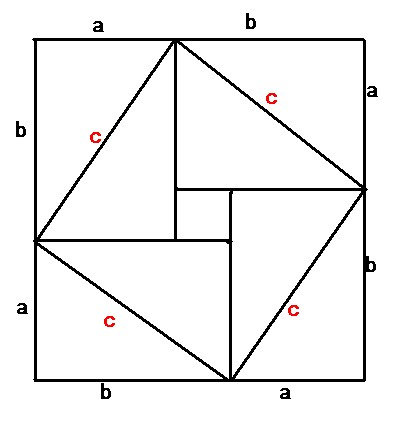
\includegraphics[width=\textwidth]{imgs/pythagorean.jpg}
        \end{figure}
    \end{minipage}%
    \hfill
    \begin{minipage}{0.4\linewidth}
        \begin{enumerate}
            \item item
            \item another
            \item more
            \begin{itemize}
                \item first
                \item second
                \item third
            \end{itemize}
        \end{enumerate}
    \end{minipage}
\end{frame}

\begin{frame}{Columns}
    \begin{columns}
        \column{0.5\textwidth}
        This is a text in first column.
        $$E=mc^2$$
        \begin{itemize}
        \item First item
        \item Second item
        \end{itemize}
        
        \column{0.5\textwidth}
        \begin{block}{first block}
            columns achieves splitting the screen
        \end{block}
        \begin{block}{second block}
            stack block in columns
        \end{block}
        
    \end{columns}
\end{frame}

\subsection{Table}

\begin{frame}{Create Tables}
    \begin{center}
        \begin{table}[!t]  
            % \caption{Three line}
            % \label{table_time}
            \begin{tabular}{ccc}  
                \toprule   
                first&second&third\\ 
                \midrule       
                1 & 2 & 3 \\ 
                4 & 5 & 6 \\ 
                7 & 8 & 9 \\
                \bottomrule  
            \end{tabular}
        \end{table}
    \end{center}
\end{frame}

\subsection{Math}

\begin{frame}{Equation1}
    A matrix in text must be set  smaller:
    $\bigl(\begin{smallmatrix}
    a&b \\ c&d
    \end{smallmatrix} \bigr)$
    to not increase leading in a portion of text.

    \[ f(n) =
    \begin{cases}
        n/2       & \quad \text{if } n \text{ is even}\\
        -(n+1)/2  & \quad \text{if } n \text{ is odd}
    \end{cases}
    \]

    $$50 apples \times 100 apples = lots of apples^2$$
\end{frame}

\begin{frame}{Equation2}
    $$\sum_{\substack{0<i<m \\ 0<j<n }} 
      P(i,j)=\int\limits_a^b\prod P(i,j)$$

    $$P\left(A=2\middle|\frac{A^2}{B}>4\right)$$

    $$( a ), [ b ], \{ c \}, | d |, \| e \|,
    \langle f \rangle, \lfloor g \rfloor,
    \lceil h \rceil, \ulcorner i \urcorner$$
\end{frame}

\begin{frame}{Equation3}
    $$Q(\alpha)=\alpha_i\alpha_jy_iy_j(x_i\cdot x_j)$$

    $$Q(\alpha)=\alpha^i\alpha^jy^{(i)}y^{(j)}(x^i\cdot x^j)$$
    
    $$\Gamma=\beta+\alpha+\gamma+\rho$$
\end{frame}



\section{Conclusion}

\begin{frame}{End}
    The last page.
\end{frame}